\documentclass{article}
\usepackage[parfill]{parskip}
\usepackage{graphicx}
\usepackage[T1]{fontenc}
\usepackage{gentium}
\usepackage{amsfonts} 

\author{Stian Onarheim}
\title{RFMA310-1 20H Diskret matematikk Hjemmeeksamen}

\begin{document}
\maketitle
\newpage
\tableofcontents
\newpage

\section{The Elgamal Encryption Algorithm}
The person who wants to receive an ecrypted text, starts by creating a private and public key. The public key consists of four elements. A cyclic group $G := (\mathbb{Z}/p)^x$ under multiplication, where $p \in Spec(\mathbb{Z})$, the group's order $q$, a generator from the group $G$, and an element $h := g^x \in G$, where $x \in G$ is the private key. The elements ($G, q, g, h$) makes the pulbic key, and is shared with the sender.

The sender will use the public key to encrypt a message $m \in G$. The sender also creates their own private key $y \in G$. The sender computes the shared secret $s := h^y \in G$. The cipertext consists of two elememts $c_1, c_2 \in G$, which are commputed as $c_1 := g^y, c_2 := m \cdot s$. The ciphertext ($c_1,c_2$) is sent to the receiver.

The receiver has now received the ciphertext ($c_1, c_2$) from the sender, and has every tool it needs to decrypt the message. It starts by computing the shared secret $s$ which was used by the sender under encryption. The sender computed it as $s := h^y \Leftrightarrow s:= g^{xy}$. Since the ciphertext element $c_1 = g^y$, the shared secret $s$ can be computed as $s := c_1^x \Leftrightarrow g^{yx}$. The plaintext $m$ is computed as $m := c_2 \cdot s^{-1}$, so the shared secret's inverse needs to be computed. Using Lagrange's theorem, the inverse can be computed as $s^{-1} := c_1^{q-x}$.

As the cyclic group $G$ has a multiplication operator, its unit element $e := 1$. The plaintext is computed as $c_2 \cdot s^{-1} \Leftrightarrow (m \cdot s) \cdot s^{-1} \Leftrightarrow m \cdot e \Leftrightarrow m$. Both parties are now left with the same plaintext message.

\section{The source code}
I have implemented Elgamal in python as it supports enormous numbers within its default libraries. Before encrypting the plaintext, I convert its characters to ASCII values and concatenates them together.\\

The message to be encrypted has to be an element of the cyclic group $G$, creating a limit to the message's length. To support longer messages, the message is divided into blocks smaller than $G$'s order. As the ASCII values varies from one to three digits, zeroes are appended at the beginning to make every value the same length. This is needed to make decryption easier. In Figure \ref{blocks}, the blue block represents an example of this padding. 

Each block is encrypted seperately with the Elgamal protocol. The ciphertexts consists of two elements ($c_1, c_2$), which combined are two times longer than the message itself. After decryption, we are left with the same blocks as before the encryption. The blocks' length are strategically a multiple of 3, which makes it easier to deconstruct them back into characters.  

\begin{figure}
    \centering
    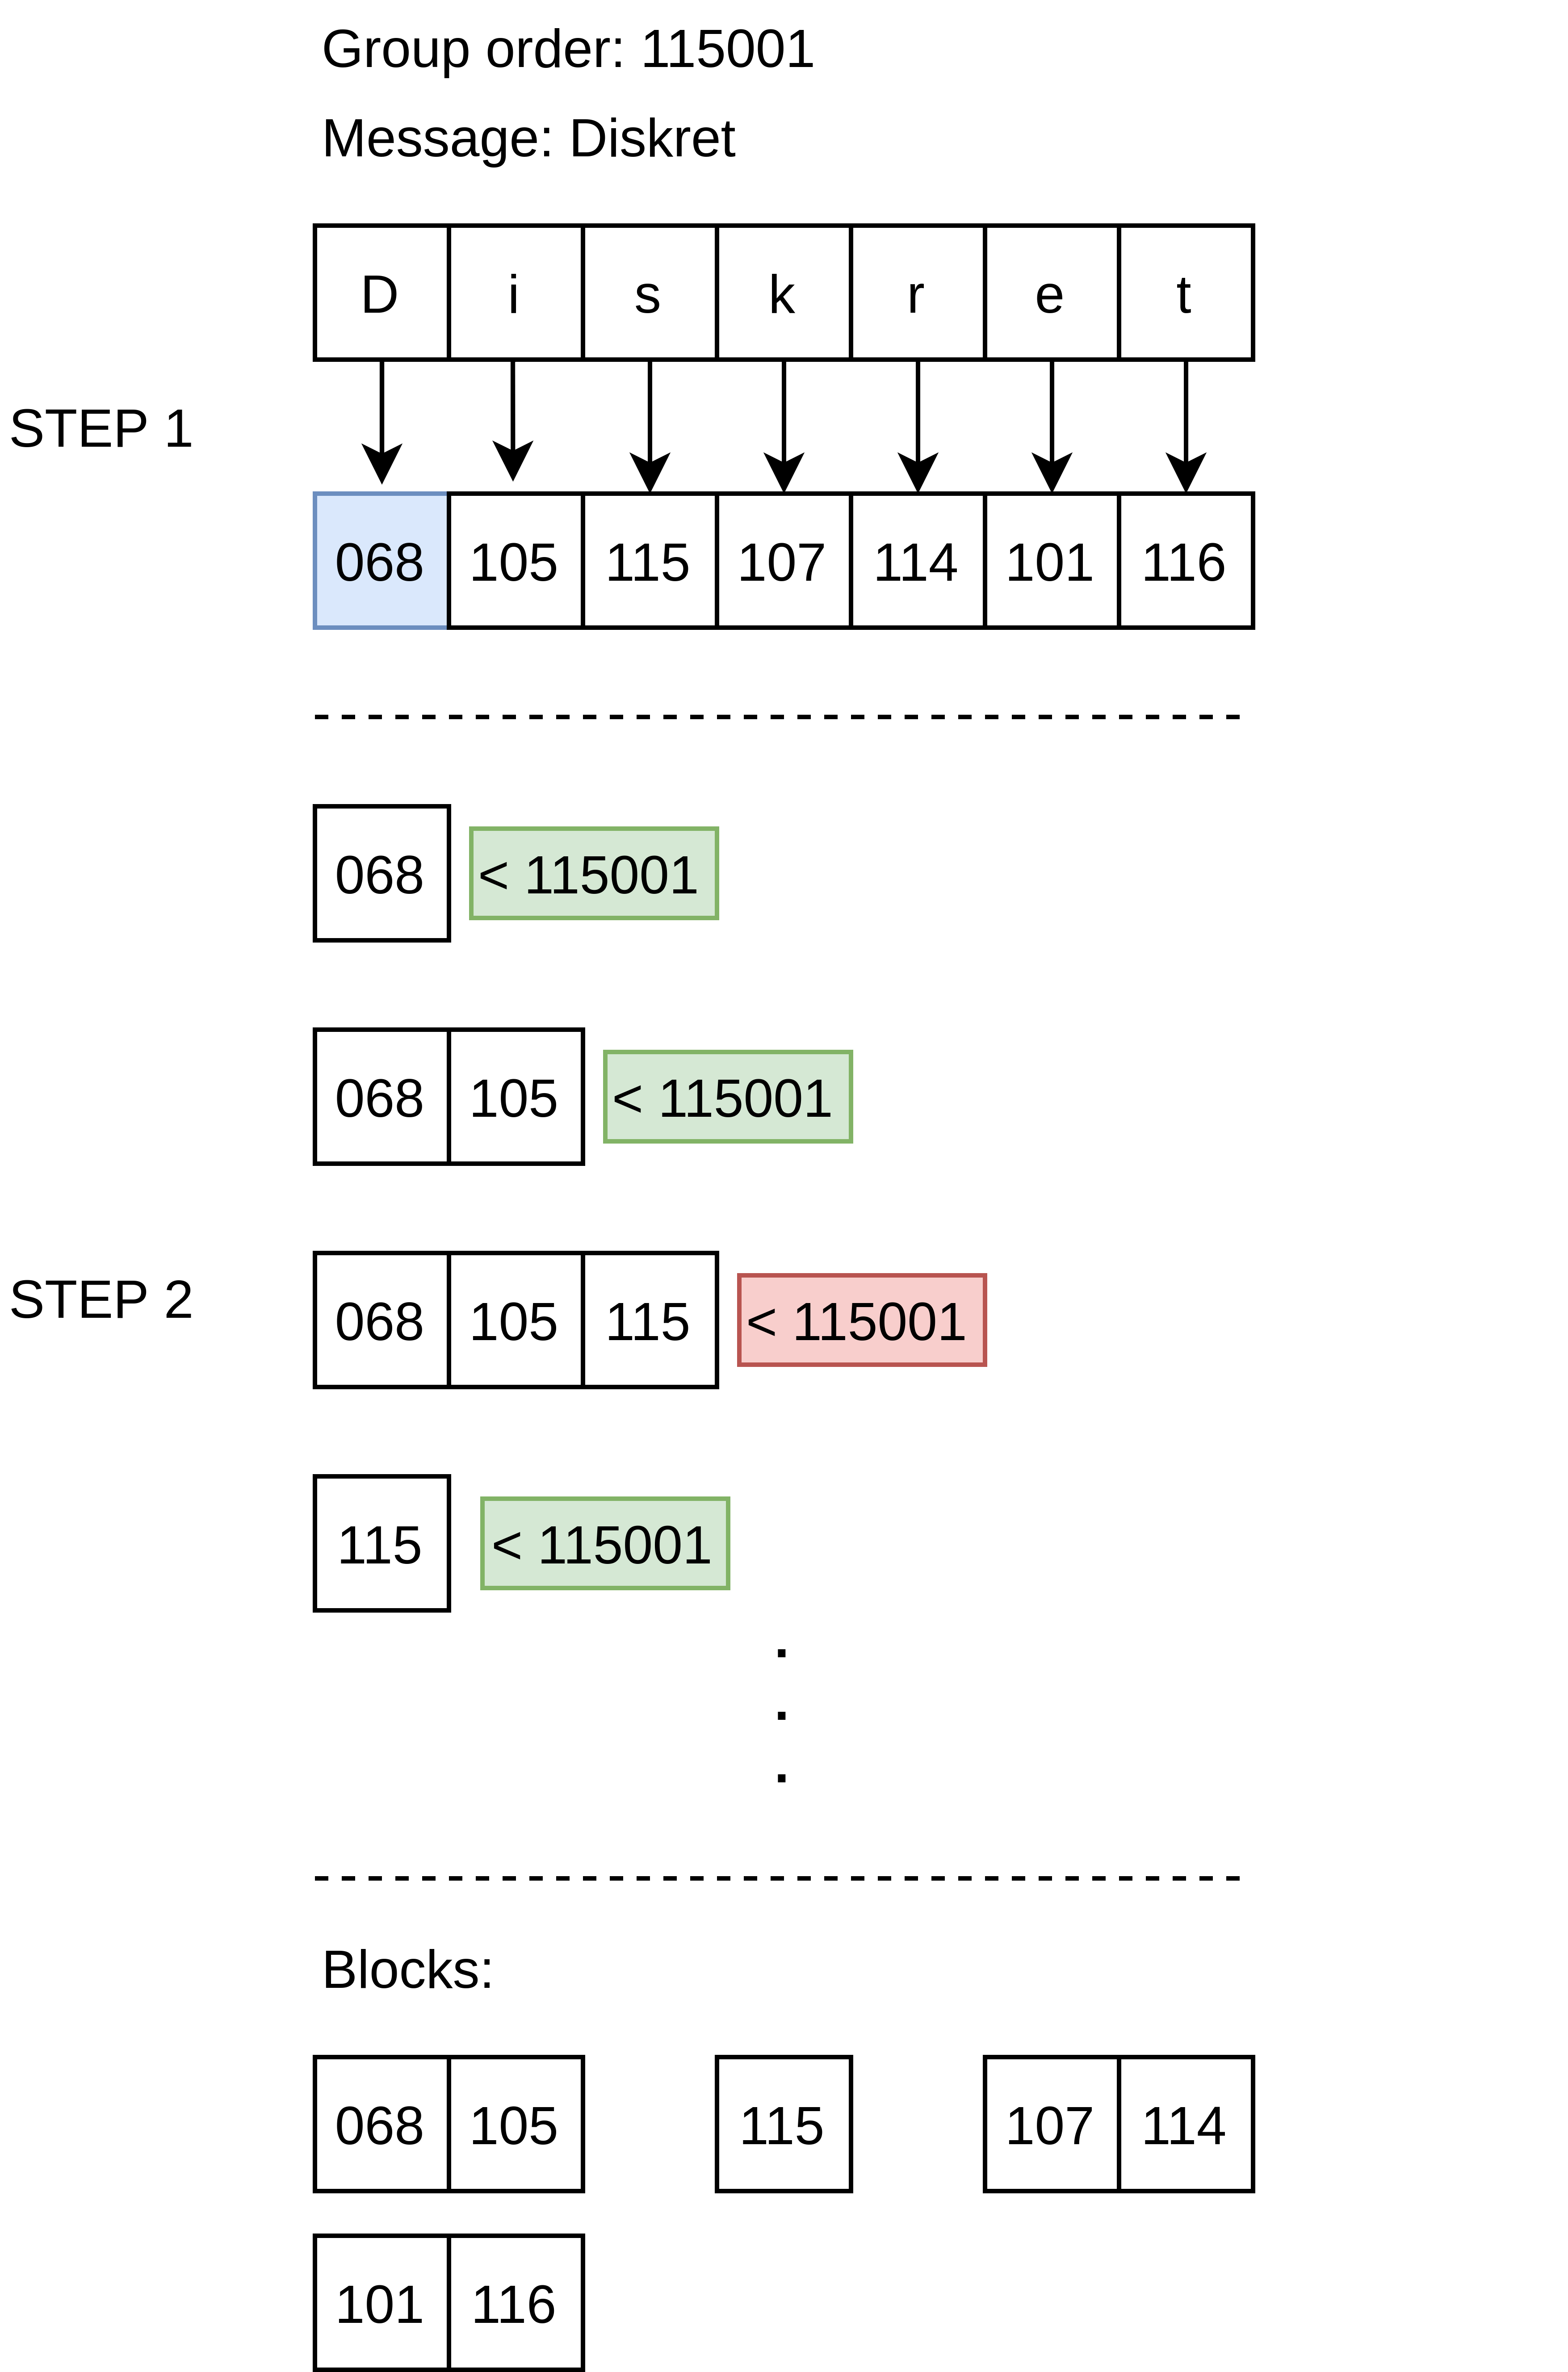
\includegraphics[scale=0.1]{img/construct-blocks.png}
    \caption{Example of constructing blocks out of the message.}
    \label{blocks}
\end{figure}
\end{document}
